\section*{CUDA Memory Management}
In most intensive applications, memory-related operations present a
bottleneck (same goes for CPU programs too I guess, they call it
the von Neumann bottleneck). Typically, your memory bandwidth
is going to be smaller than your FLOPS, and in the worst case your
FLOPS count will be capped by the memory bandwidth. This should not
happen too much because GPU is a latency-hiding architecture - large
latency memory accesses are hidden by high throughput execution.

Which is why here also we have caches, along with larger registers.
Take a look at figure \ref{fig:figures-memory-png}. Each memory
bandwidth is orders of magnitude different.

\begin{figure}[h]
    \centering
    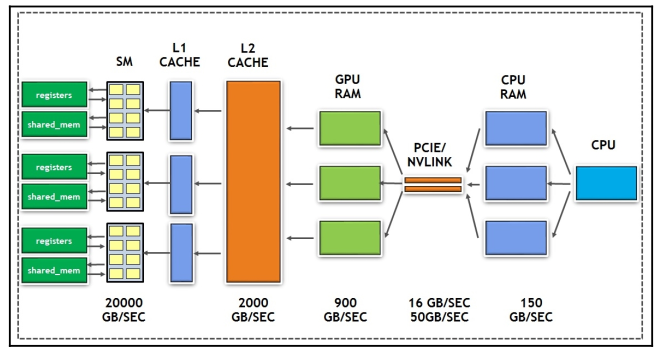
\includegraphics[width=0.8\textwidth]{figures/memory.png}
    \caption{Memory pathways in a typical host-device machine with memory bandwidths(taken
    from the book `Learn CUDA Programming' by Packtpub)}
    \label{fig:figures-memory-png}
\end{figure}

The memory hierarchy in a CUDA device (and in any typical GPU) is
a bit more involved than that of a PC host.
\begin{figure}[h]
    \centering
    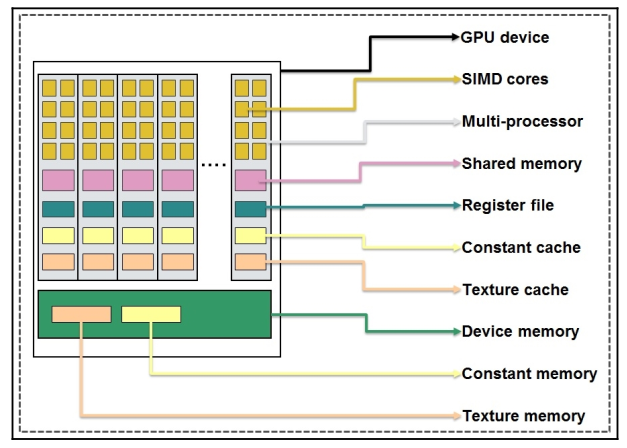
\includegraphics[width=0.8\textwidth]{figures/mem-hierarchy.png}
    \caption{Different types of memory present in a typical GPU}
    \label{fig:figures-mem-hierarchy-png}
\end{figure}

One can optimally utilize different types of GPU memories.
\begin{itemize}
    \item Global memory
    \item Shared memory
    \item Read-only data/cache
    \item Pinned memory
    \item Unified memory
\end{itemize}

\subsection*{Profiling Tools}
The CUDA Toolkit have the following main tools
\begin{itemize}
    \item nvcc - the compiler
    \item cuobjdump - similar to objdump
    \item nvdisasm - disassembler
    \item nvprune - pruning tool
    \item nsight (???)
    \item nvvp - visual profiler
    \item nvprof - command line profiler
    \item cuda-memcheck
\end{itemize}

\texttt{nvvp} is a full-fledged GUI application, complete with the
Autodesk-like splash screen :puke-emoji:

Go and read the man pages.



